\documentclass[conference]{IEEEtran}
\IEEEoverridecommandlockouts
% The preceding line is only needed to identify funding in the first footnote. If that is unneeded, please comment it out.
\usepackage{cite}
\usepackage{amsmath,amssymb,amsfonts}
\usepackage{algorithmic}
\usepackage{graphicx}
\usepackage{textcomp}
\usepackage{xcolor}
\usepackage{mathtools}
\usepackage{tabu}
\usepackage{subcaption}
\DeclareMathOperator*{\argmax}{argmax} % thin space, limits underneath in displays
\def\BibTeX{{\rm B\kern-.05em{\sc i\kern-.025em b}\kern-.08em
    T\kern-.1667em\lower.7ex\hbox{E}\kern-.125emX}}
\begin{document}
\title{Estimation of Finite Generalized Gaussian Mixture Models based on the Variational Expectation Maximization Algorithm\\
% {\footnotesize \textsuperscript{*}Note: Sub-titles are not captured in Xplore and
% should not be used}
% \thanks{Identify applicable funding agency here. If none, delete this.}
% }
}
\author{\IEEEauthorblockN{1\textsuperscript{st} Srikanth Amudala}
\IEEEauthorblockA{\textit{Concordia Institute for Information Systems Engineering} \\
\textit{Concordia University}\\
Montreal, Canada \\
srikanth.amudala@mail.concordia.ca}
\and
\IEEEauthorblockN{2\textsuperscript{nd} Given Name Surname}
\IEEEauthorblockA{\textit{dept. name of organization (of Aff.)} \\
\textit{name of organization (of Aff.)}\\
City, Country \\
email address}
\and
\IEEEauthorblockN{3\textsuperscript{rd} Given Name Surname}
\IEEEauthorblockA{\textit{dept. name of organization (of Aff.)} \\
\textit{name of organization (of Aff.)}\\
City, Country \\
email address}
\and
\IEEEauthorblockN{4\textsuperscript{th} Nizar Bouguila}
\IEEEauthorblockA{\textit{Concordia Institute for Information Systems Engineering} \\
\textit{Concordia University}\\
Montreal, Canada \\
nizar.bouguila@concordia.ca}
}
\maketitle

\begin{abstract}
    This paper presents a variational inference method to analyze finite generalized Gaussian mixture models (GGMM) which incorporate several standard mixtures widely used in signal and image processing applications, such as Laplace and Gaussian. Our work is motivated with the fact that the generalized Gaussian distribution (GGD) can be applied on different types of data due to its shape flexibility. We present a method to evaluate the posterior distribution and Bayes estimators using variational expectation-maximization algorithm. 
    The algorithm is based on treating the shape parameter as a variable. Subsequently using Binomial Expansion with two cases, we estimate the expectation of the distibutions with power parameter.
    % On this basis, the variational E-step and the variational M-step are performed alternatively to infer the posteriors of the variables and estimate the parameters. 
    The effective number of components of the GGMM are determined automatically. The experimental results demonstrate the effectiveness of the proposed algorithm by applying it to
    binary classification in medical, astrological, and image segmentation applications; while comparing it to different other approaches.    
\end{abstract}

% \begin{IEEEkeywords}
% component, formatting, style, styling, insert
% \end{IEEEkeywords}

\section{Introduction}
Statistical inference plays a vital role in many research areas such as image segmentation, signal processing, and pattern recognition. In particular, mixture models are probabilistic models representing the distribution of such population. Challenges in fitting finite mixture models include identifying the appropriate probability density function as well as the corresponding right number of components to represent a populations. 
Gaussian distribution is a well-known distribution,
which has been widely used and studied with success for many applications involving computer vision, machine learning, image processing and statistical analysis.
% which has to happen the most used and well-fitted distribution with the limitation of the symmetric shape of the Gaussian component density. However, many statistical applications like signal processing or image segmentation where there a tailed peek or asymmetric shape which would require many components for a GMM to account for such a distribution is not feasible.
However, considering many statistical applications like signal processing and image segmentation, Gaussian distribution fails to fit different shapes of data.

Recently alternative techniques have been reported in the literature to resolve the Gaussian assumption limitation. 
A generalized Gaussian distribution (GGD) has been proposed
to provide more flexibility, thanks to a new parameter called shape parameter.  
The GGD has three special cases with respect to the varying shape parameter the Laplacian, the Gaussian, and the asymptotically uniform distributions. 

For instance, generalized Gaussain mixture model (GGMM) has been used in \cite{n15} for buffer control, in \cite{n16, n17, n18} for texture classification and retrieval, in \cite{n27, n28, n29} for video and image segmentation, in \cite{n13} for multiresolution transmission of high-definition video, in \cite{n30} for SAR images statistics modeling, in \cite{n14} for subband decomposition of video,   in \cite{n19} for denoising applications, in \cite{n20, n21} for data and image compression, in \cite{n22} for edge modeling, in \cite{n23, n24} for image thresholding, in \cite{n12, n4} to fit subband histograms, in \cite{n25, n26} for speech modeling,  and in \cite{n31} for multichannel audioresynthesis.
Several methods have been proposed to estimate the parameters of GGMM such as entropy matching estimation \cite{n34, n26} and maximum likelihood estimation \cite{n32, n16, n35, n36, n10} with a deterministic approach where a single distribution is considered. A deterministic approach involves using the Expectation Maximization (EM) algorithm which has gained attention in recent times with its lower computational time. However, the EM algorithm is known for its convergence at local maxima and the tendency to overfit the model.

An alternative technique that has been gaining attention in the literature is the Bayesian method, for which the Markov chain Monte Carlo (MCMC) algorithm has been proposed in \cite{nb1}. Although the MCMC algorithm yields better results for the inference of the GGMM, it is computationally intensive to evaluate the simulation-based estimator due to the Gibbs and Metropolis Hastings sampling.

We propose a Bayesian inference approach for the GGMM within the framework of Variational Expectation Maximization (VEM) \cite{g1}. By considering possible distributions we assign appropriate priors to the mean and the precision of GGMM. We do not assign any prior distribution to the shape parameter of the GGMM in order to appropriately derive closed form expressions. 
With the well defined prior distributions, the lower bound of the variational objective function is constructed. This facilitates the derivation of the closed form updates in the variational expectation step (VE-step).
Adopting the single-step update of Newton's method from \cite{g2}, the closed-form updates for the power parameters are achieved in the variational maximization step (VM-step).
By performing alternatively the VE-step and the VM-step, all the parameters of the GGMM are updated.

Experiments are performed based on synthetic and image data sets to verify the effectiveness of the proposed method.


\section{Generalized Gaussian Mixture Model and the Variational estimate}

\subsection{Generalized Gaussian Mixture Model}
The one-dimensional GGMM for a variable $X \epsilon R $ with parameters $\mu, \tau, \lambda$ is defined as follows:
\begin{equation*}
    \begin{split}
        P(X|\mu, \tau, \lambda) &= \frac{\lambda  \tau^\frac{1}{\lambda}}{2\Gamma(\frac{1}{\lambda})}
          e^{-\tau  |(X-\mu)|^{\lambda}}    \\
          \text{where, }
        \tau &= \Bigg({\frac{1}{\sigma} \sqrt{\frac{\Gamma(\frac{3}{\lambda})}{\Gamma(\frac{1}{\lambda})}}}\Bigg)^\lambda
    \end{split}
    \end{equation*}

$\Gamma(.)$ denotes the gamma function given by $\Gamma(z) = \int_{0}^{\infty}p^{z-1}e^{-p} dp$, where $z$ and $p$ are real variables.\\
The parameters $\mu, \sigma, \lambda$  denote the mean, standard deviation and the shape parameter, respectively. The parameter $\lambda$ controls the shape of the probability density function.
The larger the value, the flatter the probability density function; and the smaller the value, the more peaked the probability density function. This means that $\lambda$ determines the decay rate of the density function. 
Note that for the two special cases, when $\lambda = 2$ and $\lambda = 1$, the GGD is reduced to the Gaussian and Laplacian distributions, respectively.
If $X$ follows a mixture of $K$ GGDs, then 
\begin{equation}
    P(X|\Theta) = \sum_{k = 1}^{K} P(X|\mu_k, \tau_k, \lambda_k)\pi_k
\end{equation}


where $\pi_k(0\leq\pi_k\leq1$ and $\sum_{k=1}^{K} \pi_k = 1)$ are the mixing weights and $p(X|\mu_k, \tau_k, \lambda_k)$ is the GGMM likelihood of component k. 
As for the symbol $\Theta = (\epsilon, \pi)$ it refers to the entire set of parameters to be estimated where $\epsilon = (\mu_1, \tau_1, \lambda_1, ..., \mu_K, \tau_K, \lambda_K)$and $\pi=(\pi_1,...,\pi_K)$. 

Considering $N$ observations,  $\mathcal{X} = (X_1, X_2, ..., X_N)$, and supposing that the number of components $K$ is known, the data likelihood is denoted as follows:
\begin{equation}
    P(\mathcal{X}|\Theta) = \prod_{n = 1}^{N}\sum_{k=1}^{K} P(X_n|\epsilon_k)\pi_k
\end{equation}
where $\epsilon_k = (\mu_k, \tau_k, \lambda_k)$. 
For each variable $X_i$, let $Z_i$  be $K$-dimensional vector known by the unobserved vector that assigns the appropriate mixture component $X_i$ belongs to. That is: $Z_{ik}$ is equal to 1 if $X_i$ belongs to class $k$ and 0, otherwise. The complete-data likelihood at that point is given by:
\begin{equation}
    P(\mathcal{X}|\Theta) = \prod_{n = 1}^{N}\sum_{k=1}^{K} (P(X_n|\epsilon_k)\pi_k)^{Z_{nk}}
\end{equation}
% where $Z =(Z_1, Z_2, ..., Z_N)$

The EM algorithm comprises of getting the mixture parameters that maximize the complete data log-likelihood function given by:
\begin{equation}
    L(\mathcal{X}, Z, \Theta) = \sum_{n = 1}^{N}\sum_{k=1}^{K} Z_{nk}\log(P(X_n|\epsilon_k)\pi_k)
\end{equation}
The assignment of $k$th component of the mixture can be denoted as follows\cite{b9}:
\begin{equation}
    \hat{Z}_{nk}^t = \frac{P^{t-1}(X_n|\epsilon_k^{t-1})p_k^{t-1}}{\sum_{k=1}^{K} P^{t-1}(X_n|\epsilon_k^{t-1}) p_k^{t-1}}
\end{equation}
where $t$ denotes the current step and $\epsilon_k^t$ and $p_j^t$ are the current estimates of the parameters.
The EM algorithm produces a sequence of estimates to the mixture parameters $\Theta^t$, for $t=0,1,...,$ until a convergence measure is fulfilled through two distinctive steps: the expectation and the maximization. The EM algorithm comprises of:
\begin{enumerate}
    \item Initialization of the mixture parameters.
    \item E-step: Compute $\hat{Z}^t_{nk}$ (Eq. (6)) using the initialized
    parameters.
    \item M-step: Update the parameters using \\
        $\hat{\Theta}^t =$ $\argmax_{z_{\Theta}}$ $L(\Theta, Z, \mathcal{X})$.
\end{enumerate}

However, the EM algorithm has some drawbacks, like convergence to local maxima due to its dependence on initialization. 
A detailed discussion of the disadvantages of the EM algorithm is in \cite{b1}.
% An extension to the EM algorithm based on the execution of the E-step by Monte Carlo, 
% called Markov chain Monte Carlo (MCEM), has been proposed in \cite{b2}. 
% Although the Markov chain Monte Carlo (MCMC) algorithm yields better results for the inference of the GGMM, it is computationally intensive to evaluate the simulation-based estimator due to the Gibbs and Metropolis sampling. 
% Moreover, both the MCMC-based method and the EM-based methods fail to address the model complexity problem (i.e., the selection of the number of components) in the GGMM.

% To achieve both the closed-form updates and the automatic determination of component number, we propose a Bayesian inference approach for the Generalized Gaussian Mixture Model within the framework of variational expectation maximization (VEM) \cite{b10}\cite{b11}.
% An efficient alternative technique that we will propose in the following is the Variational approach which has received a lot of attention in recent times.
\subsection{Variational Estimation of the GGMM}

We have proposed a variational inference approach for the GGMM within the framework of VEM \cite{b10} \cite{Bishop} to achieve the closed form updates and automatic determination of number of mixture components by 
optimizing the Kullback–Leibler (KL) divergence between the true posterior $p$ and the approximate distribution $q$ \cite{Bishop}.
The smaller KL divergence, the stronger is the relationship between the distributions.
\begin{equation}
    \begin{split}\label{kl}
    KL(p\parallel q) & = - \int q(Z) \ln\{\frac{p(Z,\mathcal{X})}{q(Z)}-\ln p(\mathcal{X})\}dZ \\ &
    = - \int q(Z) \ln\{\frac{p(Z,\mathcal{X})}{q(Z)}\}dZ + \ln p(\mathcal{X})
    \end{split}
 \end{equation}
 In order to calculate the KL divergence, we need to calculate the evidence $\ln p(X)$ which is hard to calculate and is one of motives behind the variational inference approach.
 Reordering Eq. (\ref{kl}), we get: 
 \begin{equation}
    \ln p(\mathcal{X}) = KL(p\parallel q) + \underbrace{\int q(Z) \ln\{\frac{p(Z,\mathcal{X})}{q(Z)}\}dZ}_\text{Evidence Lower Bound}
 \end{equation}
Maximizing the Evidence Lower Bound (ELBO) is same as minimizing the KL divergence. 
By applying Jensen's inequality, ELBO serves as a lower-bound for the log-evidence, $\ln p(X) \geq$ ELBO$(q)$ for any $q(Z)$, which is
the approximate of the posterior.  
In order to maximize ELBO, we need to choose a variational family $q$.
The complexity of the family determines the complexity of the optimization allowing it to be flexible in providing appropriate approximation to the true posterior distribution.

% We introduce priors to the paraeters $\mu, \tau, \lambda$ and $\pi$ by choosing 
% a Gaussian distribution for the mean $\mu$, 
% and a Gamma distribution for precision and shape parameters $\tau$ and $\lambda$ respectively, leading to the following equations:
% \begin{equation}
% p(\mu)= \prod_{k=1}^{K} N(\mu_k|m_0,s_0^{-1})%= (\frac{v_0}{2\pi})^{\frac{N}{2}}\text{exp}\{-\frac{v_0\sum_{k=1}^{K}(\mu_k - m_0)^2}{2}\}
% \end{equation}
% \begin{equation}
% p(\tau)= \prod_{k=1}^{K} Gam(\tau_{k}|\alpha_0,\beta_0)%= \frac{b_0^{a_0}}{\Gamma(a_{0})}\prod_{k=1}^{K}\tau_{l_k}^{a_0-1}\text{exp}\{-b_0\tau_{l_k}\}
% \end{equation}
% \begin{equation}
% p(\lambda)= \prod_{k=1}^{K} Gam(\tau_{\lambda_k}|\alpha_{0_\lambda},\beta_{0_\lambda})%= \frac{c_0^{d_0}}{\Gamma(c_{0})}\prod_{k=1}^{K}\tau_{r_k}^{c_0-1}\text{exp}\{-d_0\tau_{r_k}\}
% \end{equation}
% We choose a Dirichlet distribution over the mixing coefficients $\pi$
% \begin{equation}
% p(\pi)= Dir(\pi|\gamma_0)=  \frac{\Gamma(\sum_{k=1}^{K} \gamma_{0})}{\prod_{k=1}^{K} \Gamma(\gamma{0})}\prod_{k=1}^{K} \pi_k^{\gamma-1}
% \end{equation}

We assign Normal priors for the distributions means, and Gamma
priors for the precision and shape parameters [47,48]:
$\mu_k \sim N(\mu| m_0, s_0^{-1}), \tau_k \sim G(\tau|\alpha_0, \beta_0), \lambda_k \sim G(\lambda|\alpha_{\lambda}, \beta_{\lambda})$ where $N(\mu| m_0, s_0^{-1})$
is the normal distribution with mean $m_0$ and precision $s_0^{-1}$, $G(\tau|\alpha_0, \beta_0)$
is the Gamma distribution with shape parameter
$\alpha_0$ and rate parameter $\beta_0$, $\lambda$, $\mu_0, s_0, \beta_0, \alpha_0$ are the 
hyperparameters of the model. A graphical model of the GGMM maybe observed in Fig. 1.
With these priors, the posterior distributions for $\mu, \tau, \lambda$ are\cite{b9} defined as
\begin{equation}
    \begin{split}
        p(\mu_k|Z, X) &\propto e ^{{-(\mu_k - \mu_0)^2 s_0/2} + \sum_{Z_{nk} = 1} - (\tau_k|X_n - \mu_k|)^{\lambda_k}}   \\
        p(\tau_k|Z, X) &\propto \alpha_k ^{\alpha_0 - 1} e ^{-\beta_0 \tau_k}\tau_k^{n_j} e ^{\sum_{Z_{nk} = 1} - (\tau_k|X_n - \mu_k|)^{\lambda_k}}   \\
        p(\lambda_k|Z, X) &\propto \lambda_k ^{\alpha_\lambda - 1} e ^{-\beta_\lambda \lambda_k}\tau_k^{n_j}(\frac{\lambda_k}{\Gamma(1/\lambda_k)})^{n_j} \\
        &e ^{\sum_{Z_{nk} = 1} - (\tau_k|X_n - \mu_k|)^{\lambda_k}}  
    \end{split}
\end{equation}
Accordingly, we can not use our posterior distributions in their current state. 


% \subsection{Proposed VE interface of GGMM}

% PDF of Generalised Gaussian Mixture model
% \begin{equation}
%     \begin{split}
%         P(X|\mu_k, \tau_k, \lambda_k) &= \frac{\lambda_k  \tau_k^\frac{1}{\lambda_k}}{2\Gamma(\frac{1}{\lambda_k})}
%           exp(-\tau_k  |(X-\mu_k)|^{\lambda_k})    \\
%         \tau &= (\frac{1}{\sigma} \sqrt(\Gamma(\frac{3}{\lambda})/\Gamma(\frac{1}{\lambda})))^\lambda
%     \end{split}
%     \end{equation}
    
    % \begin{equation}
    % \tau = (\frac{1}{\sigma} * \sqrt(\Gamma(\frac{3}{\lambda})/\Gamma(\frac{1}{\lambda})))^\lambda
    % \end{equation}

    In order to formulate  the variational inference learning model, we write down
the joint distribution of all of the random variables considering all parameters are independent 
\begin{equation}
    p(X, Z, \pi, \mu, \tau, \lambda) = p(X|Z, \mu, \tau, \lambda)p(Z|\pi)p(\pi)p(\mu)p(\tau)p(\lambda)
\end{equation}
\begin{figure}[h!]
    \begin{center}
        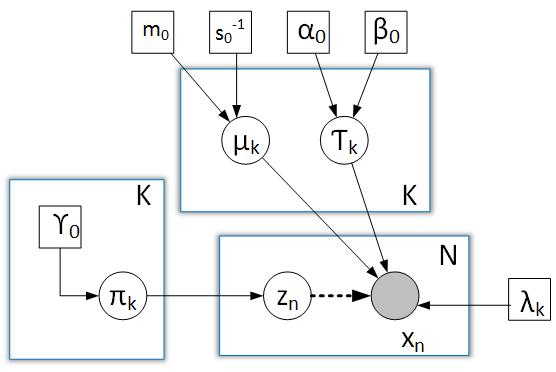
\includegraphics[width=0.7\linewidth]{imgresults/model.jpeg}
        \caption{Graphical model for the VGGM. 
        The filled circle, unfilled circles and squares represent observations, random variables, and parameters, respectively. The dependency among the variables is represented by directional arrows.}
        \label{VGGM Graphical Model}    
    \end{center}
\end{figure}

Because of the nonlinearity of the shape parameter, the conjugate prior distribution can not be directly found. Therefore, we considered using the Taylor approximation to find an 
approximate lower bound of the complete-data log-likelihood function to determine whether there is the appropriate prior distribution in the exponential family. 

But being a negative second order derivative which leads the function $q(\lambda)$ to be concave, resulting in an upper bound rather than a lower bound; which is required.
Hence, we consider $\lambda$ as a parameter and it is not assigned a prior distibution\cite{b5}.
The conjugate exponential priors for $\mu$ and $\tau$ are Normal and Gamma distibutions. Therefore, we specify all the priors according to
\begin{equation}
    \mu_k \sim N(\mu| m_k, s_k^{-1})   
\end{equation}
\begin{equation}
    \tau_k \sim G(\tau|\alpha_k, \beta_k)    
\end{equation}
We now consider a variational distribution which factorizes between the latent
variables and the parameters
\begin{equation}
    q(Z, \pi, \mu, \tau, \lambda) = q(Z)q(\pi, \mu, \tau, \lambda)
\end{equation}

\begin{equation}
    \ln q^\star(Z) = \mathop{\mathbb{E}_{\mu, \tau, \pi}}[\ln p(X, \pi,\mu, \tau, \lambda)] + const.
\end{equation}
\begin{equation}
    \begin{split}
        \ln q^\star(Z) = \mathop{\mathbb{E_\pi}}[\ln p(Z|\pi)]+\mathop{\mathbb{E_{\mu, \tau}}}[\ln p(X|Z,\mu, \tau, \lambda)] + const.
    \end{split}
\end{equation}
where, $\mathbb{E}$ represents the expectation.
Substituting the two conditional distributions, and absorbing any terms that are independent of Z into the additive constant, we have
\begin{equation}
    \ln q^\star(Z) =  \sum_{\mathclap{n=1}}^{N} \sum_{\mathclap{k=1}}^{K}z_{nk} \ln \rho_{nk} + const
\end{equation}
where we define
\begin{equation}
    \begin{split}\label{rownk}
        \ln \rho_{nk} = &\mathop{\mathbb{E}}[\ln \pi_k] + \mathop{\mathbb{E}}[\frac{1}{\lambda_k} \ln \tau_k + \ln \lambda_k - \ln 2\Gamma(1/\lambda_k)\\
        & - \tau_k |X_n - \mu_k|^{\lambda_k}]_{\mu, \tau}    
    \end{split}
\end{equation}

Normalizing the distribution, noting for each value of $n$ the values of $Z_{nk}$ are binary and add up to 1 over all values of $k$, we obtain
\begin{equation}
    q^\star(Z) = \prod_{n=1}^{N}\prod_{k=1}^{K} r_{nk}^{z_{nk}}
\end{equation}
where
\begin{equation}\label{rnk}
    r_{nk} = \frac{\rho_{nk}}{\sum_{k=1}^{K}\rho_{nk}}
\end{equation}

We see that the optimal solution for the factor $q(Z)$ takes the same functional form
as the prior $p(Z|\pi)$. Note that because $\rho_{nk}$ is given by the exponential of a real
quantity, the quantities $\rho_{nk}$ will be non-negative and will sum to one, as required.
For the discrete distribution $q^\star(Z)$ we have the standard result from which we see that
\begin{equation}
    \mathop{\mathbb{E}}[z_{nk}] = r_{nk}
\end{equation}
$r_{nk}$ are playing the role of responsibilities and the sum of all the responsibilities for the respective cluster $k$ is given by $N_k$.
\begin{equation}
    N_k = \sum_{\mathclap{n=1}}^{N}r_{nk}
\end{equation}
Similarly, the factor  in the variational posterior distribution $q(\pi, \mu, \tau, \lambda) $
\begin{equation}
    \begin{split}
        \ln q^\star (\pi, \mu, \tau, \lambda) = \ln q(\pi) +  \sum_{k=1}^{K} q(\mu_k, \tau_k, \lambda_k)
    \end{split}
\end{equation}
We observe that this expression decomposes into a sum of
terms involving only $\pi$ together with terms only involving $\mu$ and $\tau$, which implies
that the variational posterior $q(\pi, \mu, \tau, \lambda)$ factorizes to give $q(\pi)q(\mu, \tau, \lambda)$.\\
\begin{equation}
    q(\pi, \mu, \tau, \lambda) = q(\pi) \prod_{k=1}^{K} q(\mu_k, \tau_k, \lambda_k)
\end{equation}

% We choose a Dirichlet distribution over the mixing coefficients $\pi$
% \begin{equation}
% p(\pi)= Dir(\pi|\gamma_0)=  \frac{\Gamma(\sum_{k=1}^{K} \gamma_{0})}{\prod_{k=1}^{K} \Gamma(\gamma{0})}\prod_{k=1}^{K} \pi_k^{\gamma-1}
% \end{equation}

Identifying the terms on the right-hand side of that depend on $\pi$, we have \\
\begin{equation}
    \ln q^\star(\pi) = (\gamma_0 - 1)\sum_{k=1}^{K}\ln \pi_k + \sum_{k=1}^{K}\sum_{n=1}^{N} r_{nk} \ln \pi_k + const
\end{equation}
Taking the exponential of both sides, we recognize $q^\star(\pi)$ as a Dirichlet distribution with parameter $\gamma$
\begin{equation}
    q^\star(\pi) =  Dir(\pi|\gamma)
\end{equation}
where $\gamma$ has components $\gamma_k$ given by
\begin{equation}\label{gammak}
    \gamma_k = \gamma_0 + N_k
\end{equation}   
    \begin{equation}
        \begin{split}
            \mathop{\mathbb{E}}[\ln \pi_k] &= \psi(\gamma_k) - \psi(\hat{\gamma})\\
            \hat{\gamma} &= \sum_{k=1}^{K} \gamma_k
        \end{split}
    \end{equation}
    The expectation of $\mu$ with prior means and precision as $m_0$ and $ s_0^{-1}$ respectively
    \begin{align}
    \begin{split}
    \mathop{\mathbb{E}}[\ln q(\mu_k)] = &\mathop{\mathbb{E}}[\sum_{\mathclap{n=1}}^{N}(-Z_{nk}\tau_k|X_n - \mu_k|^{\lambda_k}) - \\
    &\frac{s_0}{2}(\mu_k - m_0)^2]
    -\frac{s_0}{2} + \sum_{\mathclap{n=1}}^{N}(r_{nk} \tau_k)
    \end{split}
    \end{align}

    
    $|X_n - \mu_k|^\lambda_k$ is expanded using the Binomial Expansion to the power 2 with the following conditions.\\
    $if(\mu_k > X_n )$
    \begin{equation}
        \begin{split}
            |\mu_k - X_n|^{\lambda_k}=&\mu_k^{\lambda_k} - \lambda_k \mu_k^{\lambda_k - 1} X_n +\\
            &\frac{\lambda_k}{2} (\lambda_k - 1) \mu_k^{\lambda_k - 2} X_n^2
        \end{split}
    \end{equation}
    $if(X_n>\mu_k)$
    \begin{equation}
        \begin{split}
            |X_n-\mu_k|^{\lambda_k} &= |X_n|^{\lambda_k}(1 - \frac{\mu_k}{X_n})^{\lambda_k},\\
            (1 - \frac{\mu_k}{X_n})^{\lambda_k} &= 1 - \lambda_k \frac{\mu_k}{X_n} + \frac{\lambda_k}{2}(\lambda_k-1) \frac{\mu_k^2}{X_n^2}
        \end{split}
    \end{equation}
    Substituting Eq. (28), Eq. (29) in Eq. (27) and comparing it to the prior distribution, we obtain
    \begin{equation}
        \begin{split}\label{mk}
            m_k = \frac{\frac{s_0m_0}{2} + p_1}
            {s_k}
        \end{split}
    \end{equation}
    \begin{equation}\label{sk}
        s_k = \frac{s_0}{2} + p_2
    \end{equation}
$p_1, p_2 $ have two different cases as follow
\[
    p_1= 
\begin{cases}
    \sum_{{n=1}}^{N}(r_{nk}\bar{\tau}_k\frac{\lambda_k}{4}(\lambda_k-1)\mu_k^{\lambda_k-3} x_n^2 + \\ 
        \sum_{{n=1}}^{N}(r_{nk}\bar{\tau}_k\frac{\lambda_k}{2}\mu_k^{\lambda_k-2}x_n))     ,& \text{if } X_n < m_k\\ \\
        \sum_{n=1}^{N}r_{nk}\bar{\tau}_k\lambda_k\frac{|x_n|^{\lambda_k}}{x_n},              & \text{otherwise}
\end{cases}
\]
\[
        p_2= 
    \begin{cases}
        \sum_{{n=1}}^{N}(r_{nk}\bar{\tau}_k\mu_k^{\lambda_k-2}),& \text{if } X_n < m_k\\ \\
        \sum_{{n=1}}^{N}(r_{nk}\bar{\tau}_k\frac{\lambda_k}{2}(\lambda_k-1)\frac{|x_n^{\lambda_k}|}{x_n^2}),              & \text{otherwise}
    \end{cases}
    \]

% \begin{equation}
%     \begin{split}
%         p1 = &-\sum_{\mathclap{n=1}}^{N}(r_{nk}\bar{\tau_k}\frac{\lambda_k}{4}(\lambda_k-1)\mu_k^{\lambda_k-3} x_n^2 + \\
%         &\sum_{\mathclap{n=1}}^{N}(r_{nk}\bar{\tau_k}\frac{\lambda_k}{2}\mu_k^{\lambda_k-2}x_n))    
%     \end{split}
% \end{equation}  
   
%     \begin{equation}
%         p2 = \sum_{\mathclap{n=1}}^{N}(r_{nk}\bar{\tau_k}\mu_k^{\lambda_k-2})
%     \end{equation}
    
%     Substituting Equation 9 in Equation 5
%     \begin{equation}
%         \begin{split}
%             m_k = \frac{\frac{s_0m_0}{2} + p1}
%             {s_k}
%         \end{split}
%     \end{equation}
%     \begin{equation}
%         p1 = \sum_{n=1}^{N}r_{nk}\bar{\tau_k}\lambda_k\frac{|x_n|^{\lambda_k}}{x_n}
%     \end{equation}
%     \begin{equation}
%         s_k = \frac{s_0}{2} + p2
%     \end{equation}
%     \begin{equation}
%         p2 = \sum_{\mathclap{n=1}}^{N}(r_{nk}\bar{\tau_k}\frac{\lambda_k}{2}(\lambda_k-1)\frac{|x_n^{\lambda_k}|}{x_n^2})
%     \end{equation}
Where, $\bar{\tau}$ represents the Expectation of $\tau$.
Similarly, the solution for $\tau$ is as follows
    \begin{equation}
        \mathop{\mathbb{E}}[\ln q(\tau_k)] = \mathop{\mathbb{E}}\bigg[\frac{\lambda_k \tau_k^{\frac{1}{\lambda_k}}}{2\Gamma(\frac{1}{\lambda_k})} e ^ {-\tau_k |X-\mu_k|^{\lambda_k}} + \ln\tau_k^{\alpha_0 - 1} - \beta_0 \tau_k\bigg]
    \end{equation}
    \begin{equation}
        \begin{split}\label{alphak}
            \alpha_k = \sum_{\mathclap{n=1}}^{N} r_{nk} + \alpha_0 - 1
        \end{split}
    \end{equation}
    
    \begin{equation}\label{betak}
        \beta_k = \beta_0 + \sum_{\mathclap{n=1}}^{N} r_{nk} \mathop{\mathbb{E}}[|X_n - \mu_k|^{\lambda_k}]
    \end{equation}
     \[
        \mathop{\mathbb{E}}|X_n - \mu_k|^{\lambda_k}=
    \begin{cases}
         |X_n|^{\lambda_k} - \lambda_k \frac{|X_n|^{\lambda_k}}{X_n} m_k + \\
            \frac{\lambda_k(\lambda_k - 1)}{2} \frac{|X_n|^{\lambda_k}}{X_n^2}(\frac{1}{s_k} + m_k^2)     ,& \text{if } X_n > \mu_k\\ \\
            \mathop{\mathbb{E}}[|\mu_k|^{\lambda_k} - \lambda_k \mu_k^{\lambda_k - 1} X_n + \\ 
            \frac{\lambda_k}{2} (\lambda_k - 1) \mu_k^{\lambda_k - 2} X_n^2],              & \text{otherwise}
        \end{cases}
    \]
    

    % \begin{equation}
    %     \begin{split}
    %         if X_n > \mu_k\\
    %         \mathop{\mathbb{E}}[|X_n - \mu_k|^{\lambda_k}] &= |X_n|^{\lambda_k} - \lambda_k \frac{|X_n|^{\lambda_k}}{X_n} m_k + \\
    %         &\frac{\lambda_k}{2} (\lambda_k - 1) \frac{|X_n|^{\lambda_k}}{X_n^2}(\frac{1}{s_k} + m_k^2)    
    %     \end{split}
    % \end{equation}
    
    % \begin{equation}
    %     \begin{split}
    %         if X_n < \mu_k\\
    %         \mathop{\mathbb{E}}[|\mu_k - X_n|^{\lambda_k}] &= \mathop{\mathbb{E}}[|\mu_k|^{\lambda_k} - \lambda_k \mu_k^{\lambda_k - 1} X_n + \\
    %         &\frac{\lambda_k}{2} (\lambda_k - 1) \mu_k^{\lambda_k - 2} X_n^2]
    %     \end{split}
    % \end{equation}
    
    \text{Then using confluent hypergeometric function}
    \begin{equation}
        \begin{split}
            \displaystyle \operatorname {\mathbb{E}} \left[|\mu_k|^{\lambda_k}\right]&=\\
            (\frac{1}{\sqrt{s_k}})^{\lambda_k}\cdot 2^{\lambda_k/2}&{\frac {\Gamma \left({\frac {1+\lambda_k}{2}}\right)}{\sqrt {\pi }}}
            {}_{1}F_{1}\left(-{\frac {\lambda_k}{2}},{\frac {1}{2}},-{\frac {1}{2}}\left({m_k}\right)^{2} s_k \right).  
        \end{split}
    \end{equation}
    % Where, $ \operatorname {\mathbb{E}} $ represents Expectation.\\
    The following equation completes the lower bound
    \begin{equation}
        \begin{split}\label{lowerbound}
         \mathcal{L}&= \mathop{\mathbb{E}}[\ln P(X|\Theta)] + \mathop{\mathbb{E}}[\ln P(Z|\pi)] +\mathop{\mathbb{E}}[\ln P(\pi)]\\
        &+ \mathop{\mathbb{E}}[\ln P(\mu)]+\mathop{\mathbb{E}}[\ln P(\tau)] -\mathop{\mathbb{E}}[\ln q(Z)]\\
        &-\mathop{\mathbb{E}}[\ln q(\pi)]-\mathop{\mathbb{E}}[\ln q(\mu)]-\mathbb{E}[\ln q(\tau)]
        \end{split}
        \end{equation}
        Given the posterior distributions from the VE-step, the VM-step updates the parameters by maximizing the approximate lower bound $\mathcal{L}$.
        To estimate the parameters of the GGMM (i.e. $\lambda$), the first-order derivative of the approximate lower bound is set to zero, leading to:
        \begin{equation}
            \begin{split}
                \frac{\partial \bar{L}(q, \Theta)}{\partial \lambda_k} &= \bar{L}_i^{'}(q, \Theta)\\
                &=\sum_{n=1}^{N}\sum_{k=1}^{K} r_{nk}(|X_n - \bar{\mu}_k|^{\lambda_k} \ln |X_n - \bar{\mu}_k|(\tau_k - \bar{\tau}_k) \\
                &- \frac{1}{\lambda_k^2} \ln \bar{\tau}_k + \frac{1}{\lambda_k} - \frac{\Gamma'(\frac{1}{\lambda_k})}{2\Gamma(\frac{1}{\lambda_k})} \\
                &+ \bar{\tau}_k|X_n - \mu_k|^{\lambda_k} \ln |X_n - \mu_k|)
            \end{split}
        \end{equation}
        The second-order derivative is given by:
        \begin{equation}
            \begin{split}
                \frac{\partial^2 \bar{L}(q, \Theta)}{\partial^2 \lambda_k} &= \bar{L}_i^{''}(q, \Theta)  \\
                &=\sum_{n=1}^{N}\sum_{k=1}^{K} r_{nk}(2 |X_n - \bar{\mu}_k|^\lambda_k \ln |X_n - \bar{\mu}_k|(\tau_k - \bar{\tau}_k) \\
                &+ \frac{2}{\lambda_k^3} \ln \bar{\tau}_k - \frac{1}{\lambda_k^2}  + \frac{1}{2}\frac{\Gamma'(\frac{1}{\lambda_k})^2}{\Gamma(\frac{1}{\lambda_k})^2}- \frac{\Gamma''(\frac{1}{\lambda_k})}{2\Gamma(\frac{1}{\lambda_k})} \\
                &+ 2\bar{\tau}_k|X_n - \mu_k|^{\lambda_k} \ln |X_n - \mu_k|)  
            \end{split}
        \end{equation}
        The shape parameter is now completed as
        \begin{equation}
            \begin{split}\label{lambda}
                \lambda_k^\star = \lambda_k + s \Delta \lambda_k   \\
                \text{where }
                \Delta\lambda_k = - \frac{L_k'(q, \Theta)}{L_k''(q, \Theta)}
            \end{split}
        \end{equation}
        \text{Here, $s$ is determined by the backtracking line search \cite{b6}}. Our complete algorithm can then be summarized as follows: 
        

\subsection*{\textbf{Algorithm}}
\begin{enumerate}
    \item Input: $X, K$, given an initial large $K$ value.
    \item Initialization: choose  $\alpha_0, \beta_0, \gamma_0, m_0, s_0 $ using K-means algorithm, $\lambda_k = 2$
    \item Compute $\alpha_k, \beta_k, \gamma_k, m_k, s_k$ $\leftarrow$ Initial values for each component.
    \item \textbf{While} $L_i - L_{i-1} <= 1e-9$ 
    \item $\quad\quad$Compute $\ln \rho_{nk}$ using Eq. (\ref{rownk})
    \item $\quad\quad$Generate the responsibilities $r_{nk}$ from Eq. (\ref{rnk})
    \item $\quad\quad$Update $\alpha_k, \beta_k, \gamma_k$ $\leftarrow$ from Eq. (\ref{alphak}), Eq. (\ref{betak}) and
    Eq. (\ref{gammak})
    \item $\quad\quad$Calculate $m_k, s_k$ from Eq. (\ref{mk}), Eq. (\ref{sk}) 
    % \[
    %     m_k= 
    % \begin{cases}
    %     Eq. (32) ,& \text{if } X_n > m_k\\
    %     Eq. (29),              & \text{otherwise}
    % \end{cases}
    % \]
    % \[
    %     s_k= 
    % \begin{cases}
    %     Eq. (33) ,& \text{if } X_n > m_k\\
    %     Eq. (30),              & \text{otherwise}
    % \end{cases}
    % \]
    \item $\quad\quad$Choose the step size s by the backtracking line search
    \item $\quad\quad$Update $\lambda_k$ using Eq. (\ref{lambda})
    \item $\quad\quad$Generate lower bound $\mathcal{L}$ using Eq. (\ref{lowerbound})
    \item $\quad\quad$Assign the cluster labels to the highest responsibilities in each row of the responsibility matrix.
    \item \textbf{end}
    
\end{enumerate}
\section{Experimental results and discussion}
\subsection{Implementation details}
In the prior distibutions for the shape parameter, the hyperparameters are set as $\alpha_0 = \mu^2/\sigma, \beta_0 = \mu/N, $ given N observations. $\lambda=2, m_0, s_0^{-1}, \gamma_0$ are initialized using K-means algorithm.
Based on these initializations, we determine the sample mean, sample precision, and shape in the $i$th initial class.
When the VEM algorithm stops, $\alpha_k, \beta_k, \gamma_k, m_k, s_k, \lambda_k$ are accepted as the hyperparameter and parameter estimates in the Variational GGMM.
\subsection{Dataset validation}
This section has two main objectives: first applying the algorithm to estimate the mixture parameters and comparing with Variational GMM.

To reach the first objective, we apply our variational GGMM (VGGMM) estimation algorithm for binary classification in medical and astrological applications involving
detection of heart diseases\footnote{https://www.kaggle.com/ronitf/heart-disease-uci.} and predicting a Pulsar Star\footnote{https://www.kaggle.com/pavanraj159/predicting-a-pulsar-star/downloads/predicting-a-pulsar-star.zip/1} and finally we apply our model in image segmentation.


    \begin{figure}[h!]
        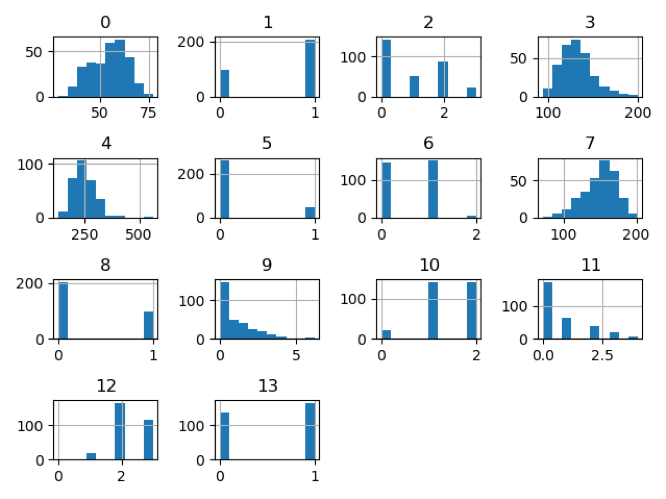
\includegraphics[width=\linewidth]{heart.png}
        \caption{Histogram of Heart Disease. Histogram-0 to Histogram-12 represent the features, Histogram-13 represents the target value with
        x-axis representing the value range and y-axis representing the frequency.}
        \label{histogram of Heart Disease data}
    \end{figure}
    \begin{figure}[h!]
        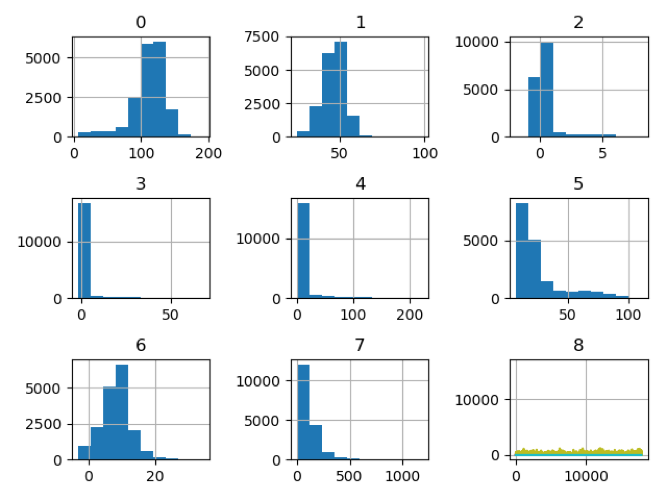
\includegraphics[width=\linewidth]{star.png}
        \caption{Histogram of Pulsar Star. Histogram-0 to Histogram-12 represent the features, Histogram-13 represents the target value with
        x-axis representing the value range and y-axis representing the frequency.}
        \label{histogram of Heart Disease data}
    \end{figure}
    
    
% \subsection{Evaluating using the two data sets}

Among the two data sets, the first one provides all the potential symptoms of a person with a positive heart disease. 
This database contains 76 attributes, but all distributed tests refer to employing a subset of 14. The objective field alludes to the presence of heart infection within the patient. Its numbers valued from 0 (no presence) to 4.
The second data set describes a sample of pulsar candidates collected during the High Time Resolution Universe Survey.
Pulsars are a rare type of Neutron star that produce radio emission detectable here on earth. They are of considerable scientific interest as probes of space-time, the inter-stellar medium, and states of matter.
It has gained popularity over recent times to label the pulsar candidates to facilitate rapid analysis. Classification systems in particular are being widely adopted, which treat the candidate data sets as binary classification problems, which is a perfect fit for our comparision.
The histograms of the input data sets have been presented in \figurename {2} and \figurename {3}. 


We have implemented our VGGMM classifer using cross validation with the split size of 4 for both the datasets. 
The label for each data point is determined with the largest component among the likelihood of the data point belonging to the classes.
Table 1, presents the model accuracy in comparison with Variational GMM.
\begin{table}[h!]
    \caption{Model accuracy comparison}
    \begin{center}
    \begin{tabular}{|c|c|c|}
    \hline
    \textbf{}&\multicolumn{2}{|c|}{\textbf{Accuracy}} \\
    \cline{2-3} 
    \textbf{\textit{Data set name}}& \textbf{\textit{VGM}}& \textbf{\textit{VGGMM}}\\
    \hline
    Heart Disease UCI& 41$\%$&69.64$\%$   \\
    \hline
    Predicting a Pulsar star& 88$\%$&93.2$\%$    \\
    \hline
    % \multicolumn{3}{l}{$^{\mathrm{a}}$Sample of a Table footnote.}
    \end{tabular}
    \label{tab1}
    \end{center}
\end{table}
\subsection{Image Segmentation}
In computer vision, Image segmentaion is the process of finding the pixels with similar characteristics and clustering them to different segments. The goal of segmentation is to find the similar pixels and represent the whole image in the form of segments with each segment representing pixels with similar characteristics making it easier for analysis \cite{b12}\cite{b13}.
\begin{figure}
    \centering
    \begin{subfigure}{.5\linewidth}
      \centering
      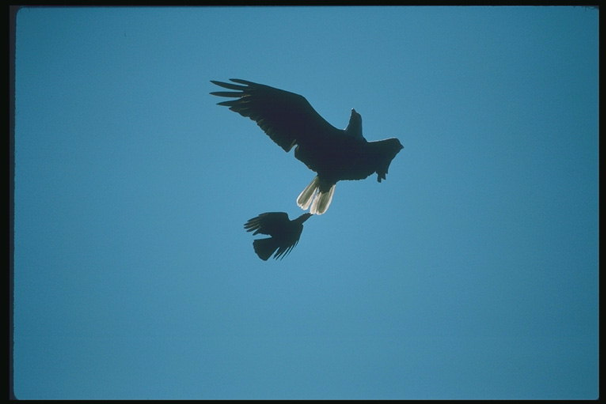
\includegraphics[width=0.9\textwidth]{imgresults/eagle_original.png}
      \caption{Original Image}
      \label{fig:sub1}
    \end{subfigure}%
    \begin{subfigure}{.5\linewidth}
        \centering
        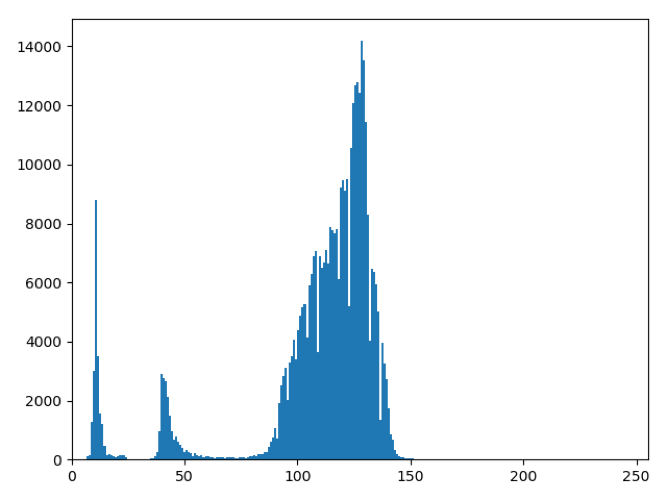
\includegraphics[width=1\textwidth]{imgresults/eagle_hist.png}
        \caption{histogram}
        \label{fig:histogram}
    \end{subfigure}
    \label{fig:sub}


    \begin{subfigure}{.5\linewidth}
        \centering
        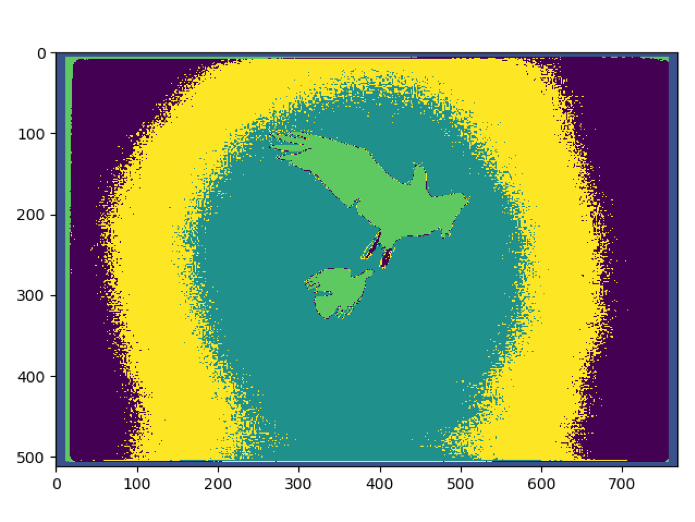
\includegraphics[width=1\textwidth]{imgresults/eagle_kmeans.png}
        \caption{K-means algorithm ($K$=5)}
        \label{fig:sub1}
      \end{subfigure}%
      \begin{subfigure}{.5\linewidth}
          \centering
          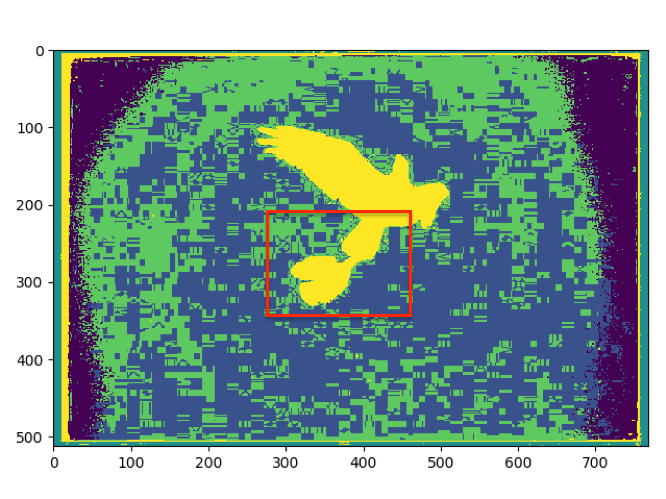
\includegraphics[width=1\textwidth]{imgresults/eagle_gmm.png}
          \caption{GMM ($K$=5)}
          \label{fig:histogram}
      \end{subfigure}
      \label{fig:sub}


    \centering
    \begin{subfigure}{.5\linewidth}
        \centering
        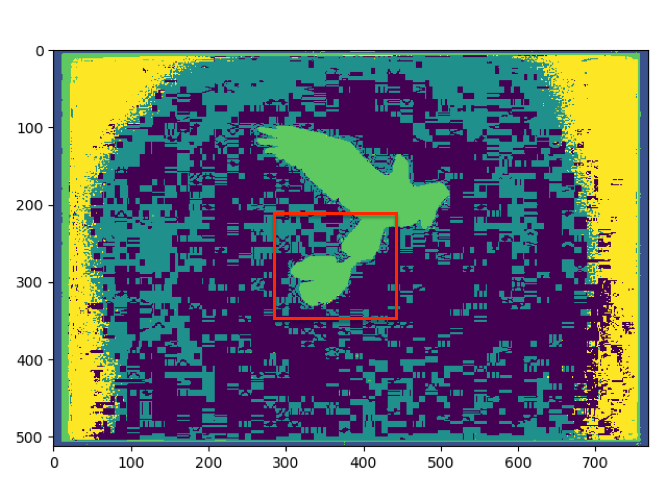
\includegraphics[width=1\textwidth]{imgresults/eagle_vgm.png}
        \caption{VGM ($K$=5)}
        \label{fig:sub1}
    \end{subfigure}%
    \begin{subfigure}{.5\linewidth}
        \centering
        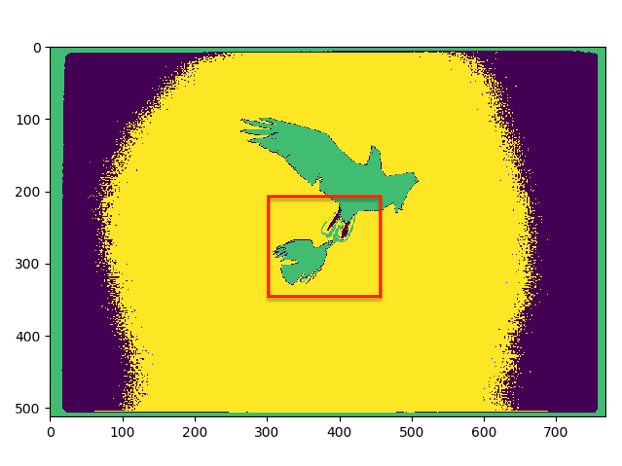
\includegraphics[width=1\textwidth]{imgresults/eagle_vggm.png}
        \caption{VGGMM ($K$=5)}
        \label{fig:sub2}
    \end{subfigure}
    \caption{Segmentation results.}
    \label{fig:eagle}
\end{figure}


%CROW

\begin{figure}
    \centering
    \begin{subfigure}{.5\linewidth}
      \centering
      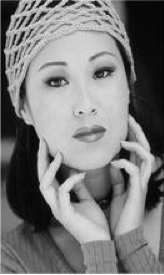
\includegraphics[height=0.7\textwidth]{imgresults/face_original.png}
      \caption{Original Image}
      \label{fig:sub1}
    \end{subfigure}%
    \begin{subfigure}{.5\linewidth}
        \centering
        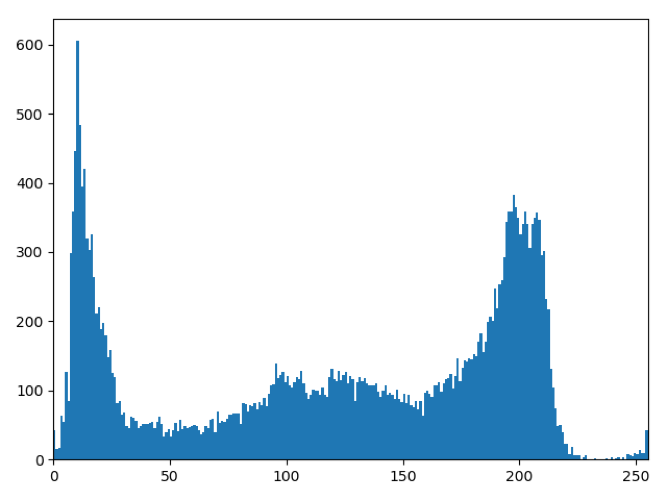
\includegraphics[width=1\textwidth]{imgresults/face_hist.png}
        \caption{histogram}
        \label{fig:histogram}
    \end{subfigure}
    \label{fig:sub}


    \begin{subfigure}{.5\linewidth}
        \centering
        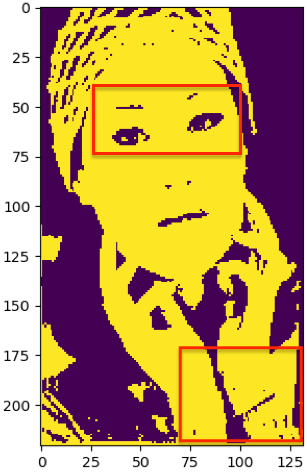
\includegraphics[height=0.7\textwidth]{imgresults/face_kmeans.png}
        \caption{K-means algorithm ($K$=2)}
        \label{fig:sub1}
      \end{subfigure}%
      \begin{subfigure}{.5\linewidth}
          \centering
          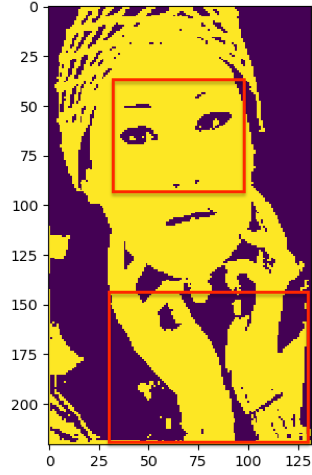
\includegraphics[height=0.7\textwidth]{imgresults/face_gmm.png}
          \caption{GMM ($K$=2)}
          \label{fig:histogram}
      \end{subfigure}
      \label{fig:sub}


    \centering
    \begin{subfigure}{.5\linewidth}
        \centering
        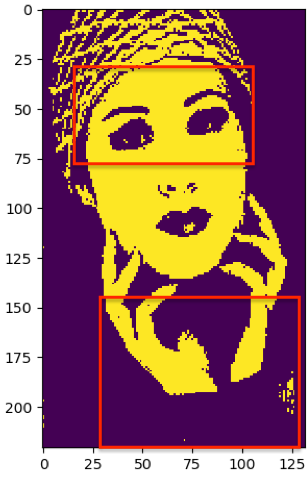
\includegraphics[height=0.7\textwidth]{imgresults/face_vgm.png}
        \caption{VGM ($K$=2)}
        \label{fig:sub1}
    \end{subfigure}%
    \begin{subfigure}{.5\linewidth}
        \centering
        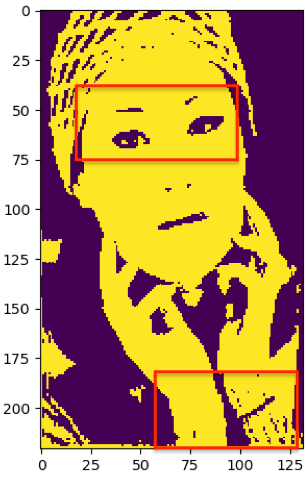
\includegraphics[height=0.7\textwidth]{imgresults/face_vggmm.png}
        \caption{VGGMM ($K$=2)}
        \label{fig:sub2}
    \end{subfigure}
    \caption{Segmentation results.}
    \label{fig:crow}
\end{figure}
In the first experiment, we chose an image (768 × 512) with two birds in the sky to show the capability to segment small objects in a large background (Fig. 4a). 
The goal was to cluster the image into two classes: the objects with two birds and the sky. 
We set the number of components, $K= 5$
Comparing the results for K-means algorithm, GMM, and VGM (Fig. 4c, Fig. 4d, Fig. 4e), there was a large misclassification of the sky and the space between the small object and the large object.
Our method, VGGMM (Fig. 4f), was able to distinguish the two birds and to detect the components effectively. Compared to the other methods, the wings, the tail of the little bird (red square) and the big bird are also shown in more details. 

In the second experiment, we performed our evaluation on a human face image (132 × 221) as shown in Fig. 5a. The goal was to segment the image into two classes. In Fig. 5b, we can she the histogram of the image. 
We set the number of componets, $K=2$,
Comparing the result with K-means algorithm, GMM, VGM methods, we noticed that K-means algorithm and GMM have similar results and were able to detect some features of the face. However, they contained only a part of the eyebrows and a part of texture of clothes rather than the whole. 
VGM was able to detect the eyebrows, but was not able to detect the texture and the hair. 

Our algorithm VGGMM (Fig. 5f), showed more details to offer more information for face recognition and image understanding.

% \begin{figure}[h!]
%     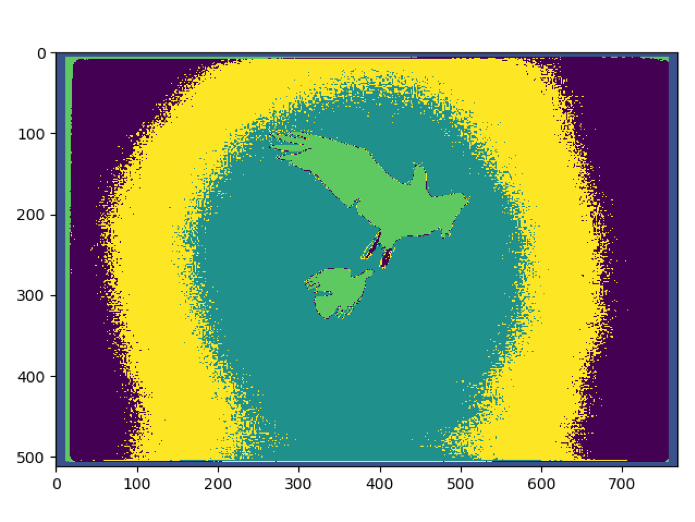
\includegraphics[width=0.5\linewidth]{imgresults/eagle_kmeans.png}
%     \caption{Histogram of Heart Disease data}
%     \label{histogram of Heart Disease data}
% \end{figure}
\section{Conclusion}
We have presented a variational inference for GGMM. The algorithm is based on treating the shape parameter as a variable. Subsequently, using Binomial Expansion with two cases, we estimate the expectation of the distibutions with power parameter. Hence, the posterior distributions of the inference can be updated by the corresponding hyperparameters.
In the VM-step, the shape parameter is updated using the single-step update of the Newton’s method.


Experimental results show the VGGM model is an accurate model for performing classification, prediction, and image segmentation by effectively estimating the parameters.
Moreover, in comparison with the VGM, the VGGM model has performed better for both classification and image segmentation. 
% in cases of the non gaussian distributed data.
% \subsection{\LaTeX-Specific Advice}

% Please use ``soft'' (e.g., \verb|\eqref{Eq}|) cross references instead
% of ``hard'' references (e.g., \verb|(1)|). That will make it possible
% to combine sections, add equations, or change the order of figures or
% citations without having to go through the file line by line.

% Please don't use the \verb|{eqnarray}| equation environment. Use
% \verb|{align}| or \verb|{IEEEeqnarray}| instead. The \verb|{eqnarray}|
% environment leaves unsightly spaces around relation symbols.

% Please note that the \verb|{subequations}| environment in {\LaTeX}
% will increment the main equation counter even when there are no
% equation numbers displayed. If you forget that, you might write an
% article in which the equation numbers skip from (17) to (20), causing
% the copy editors to wonder if you've discovered a new method of
% counting.

% {\BibTeX} does not work by magic. It doesn't get the bibliographic
% data from thin air but from .bib files. If you use {\BibTeX} to produce a
% bibliography you must send the .bib files. 

% {\LaTeX} can't read your mind. If you assign the same label to a
% subsubsection and a table, you might find that Table I has been cross
% referenced as Table IV-B3. 

% {\LaTeX} does not have precognitive abilities. If you put a
% \verb|\label| command before the command that updates the counter it's
% supposed to be using, the label will pick up the last counter to be
% cross referenced instead. In particular, a \verb|\label| command
% should not go before the caption of a figure or a table.

% Do not use \verb|\nonumber| inside the \verb|{array}| environment. It
% will not stop equation numbers inside \verb|{array}| (there won't be
% any anyway) and it might stop a wanted equation number in the
% surrounding equation.

% \subsection{Some Common Mistakes}\label{SCM}
% \begin{itemize}
% \item The word ``data'' is plural, not singular.
% \item The subscript for the permeability of vacuum $\mu_{0}$, and other common scientific constants, is zero with subscript formatting, not a lowercase letter ``o''.
% \item In American English, commas, semicolons, periods, question and exclamation marks are located within quotation marks only when a complete thought or name is cited, such as a title or full quotation. When quotation marks are used, instead of a bold or italic typeface, to highlight a word or phrase, punctuation should appear outside of the quotation marks. A parenthetical phrase or statement at the end of a sentence is punctuated outside of the closing parenthesis (like this). (A parenthetical sentence is punctuated within the parentheses.)
% \item A graph within a graph is an ``inset'', not an ``insert''. The word alternatively is preferred to the word ``alternately'' (unless you really mean something that alternates).
% \item Do not use the word ``essentially'' to mean ``approximately'' or ``effectively''.
% \item In your paper title, if the words ``that uses'' can accurately replace the word ``using'', capitalize the ``u''; if not, keep using lower-cased.
% \item Be aware of the different meanings of the homophones ``affect'' and ``effect'', ``complement'' and ``compliment'', ``discreet'' and ``discrete'', ``principal'' and ``principle''.
% \item Do not confuse ``imply'' and ``infer''.
% \item The prefix ``non'' is not a word; it should be joined to the word it modifies, usually without a hyphen.
% \item There is no period after the ``et'' in the Latin abbreviation ``et al.''.
% \item The abbreviation ``i.e.'' means ``that is'', and the abbreviation ``e.g.'' means ``for example''.
% \end{itemize}
% An excellent style manual for science writers is \cite{b7}.

% \subsection{Authors and Affiliations}
% \textbf{The class file is designed for, but not limited to, six authors.} A 
% minimum of one author is required for all conference articles. Author names 
% should be listed starting from left to right and then moving down to the 
% next line. This is the author sequence that will be used in future citations 
% and by indexing services. Names should not be listed in columns nor group by 
% affiliation. Please keep your affiliations as succinct as possible (for 
% example, do not differentiate among departments of the same organization).

% \subsection{Identify the Headings}
% Headings, or heads, are organizational devices that guide the reader through 
% your paper. There are two types: component heads and text heads.

% Component heads identify the different components of your paper and are not 
% topically subordinate to each other. Examples include Acknowledgments and 
% References and, for these, the correct style to use is ``Heading 5''. Use 
% ``figure caption'' for your Figure captions, and ``table head'' for your 
% table title. Run-in heads, such as ``Abstract'', will require you to apply a 
% style (in this case, italic) in addition to the style provided by the drop 
% down menu to differentiate the head from the text.

% Text heads organize the topics on a relational, hierarchical basis. For 
% example, the paper title is the primary text head because all subsequent 
% material relates and elaborates on this one topic. If there are two or more 
% sub-topics, the next level head (uppercase Roman numerals) should be used 
% and, conversely, if there are not at least two sub-topics, then no subheads 
% should be introduced.

% \subsection{Figures and Tables}
% \paragraph{Positioning Figures and Tables} Place figures and tables at the top and 
% bottom of columns. Avoid placing them in the middle of columns. Large 
% figures and tables may span across both columns. Figure captions should be 
% below the figures; table heads should appear above the tables. Insert 
% figures and tables after they are cited in the text. Use the abbreviation 
% ``Fig.~\ref{fig}'', even at the beginning of a sentence.

% \begin{table}[htbp]
% \caption{Table Type Styles}
% \begin{center}
% \begin{tabular}{|c|c|c|c|}
% \hline
% \textbf{Table}&\multicolumn{3}{|c|}{\textbf{Table Column Head}} \\
% \cline{2-4} 
% \textbf{Head} & \textbf{\textit{Table column subhead}}& \textbf{\textit{Subhead}}& \textbf{\textit{Subhead}} \\
% \hline
% copy& More table copy$^{\mathrm{a}}$& &  \\
% \hline
% \multicolumn{4}{l}{$^{\mathrm{a}}$Sample of a Table footnote.}
% \end{tabular}
% \label{tab1}
% \end{center}
% \end{table}

% \begin{figure}[htbp]
% %\centerline{\includegraphics{fig1.png}}
% \caption{Example of a figure caption.}
% \label{fig}
% \end{figure}

% Figure Labels: Use 8 point Times New Roman for Figure labels. Use words 
% rather than symbols or abbreviations when writing Figure axis labels to 
% avoid confusing the reader. As an example, write the quantity 
% ``Magnetization'', or ``Magnetization, M'', not just ``M''. If including 
% units in the label, present them within parentheses. Do not label axes only 
% with units. In the example, write ``Magnetization (A/m)'' or ``Magnetization 
% \{A[m(1)]\}'', not just ``A/m''. Do not label axes with a ratio of 
% quantities and units. For example, write ``Temperature (K)'', not 
% ``Temperature/K''.

\section*{Acknowledgment}

The completion of this research was made possible thanks to the Natural Sciences and Engineering Research Council of Canada (NSERC). 

% \begin{thebibliography}{00}
% \bibitem{b1} G.J. McLachlan, T. Krishnan, The EM Algorithm and Extensions, Wiley-Interscience, New York, 1997.
% \bibitem{b2} G.C.G. Wei, M.A. Tanner, A Monte Carlo implementation of the
% EM algorithm and the poor man’s data augmentation algorithms,
% Journal of the American Statistical Association 85 (1990) 699–704.
% \bibitem{b3} W. Pieczynski, Statistical image segmentation, Machine Graphics
% and Vision 1 (1–2) (1992) 261–268.
% \bibitem{b4} J.P. Delmas, An equivalence of the EM and ICE algorithm for
% exponential family, IEEE Transactions on Signal Processing 45 (10)
% (1997) 2613–2615.
% \bibitem{b5} Bayesian estimation of generalized Gamma mixture model based 
% on variational EM algorithm.
% \bibitem{b6} S. Boyd, L. Vandenberghe, Convex Optimization, Cambridge University Press,
% Cambridge, 2004.
% \bibitem{b7} https://www.kaggle.com/ronitf/heart-disease-uci.
% \bibitem{Bishop} Christopher M. Bishop, Pattern Recognition and Machine Learning.
% \bibitem{b8} https://www.kaggle.com/pavanraj159/predicting-a-pulsar-star/downloads/predicting-a-pulsar-star.zip/1.
% \bibitem{b9} Bayesian learning of finite generalized Gaussian mixture models on images.
% \bibitem{b10} D.G. Tzikas, A.C. Likas, N.P. Galatsanos, The variational approximation for Bayesian inference, IEEE Signal Process. Mag. 25 (6) (2008) 131–146.
% \bibitem{b11} C.M. Bishop, Pattern Recognition and Machine Learning, Springer-Verlag, New York, 2006.


% \bibitem{b12} Linda G. Shapiro and George C. Stockman (2001): “Computer Vision”, pp 279-325, New Jersey, Prentice-Hall, ISBN 0-13-030796-3.


% \bibitem{b13} Barghout, Lauren, and Lawrence W. Lee. "Perceptual information processing system." Paravue Inc. U.S. Patent Application 10/618,543, filed July 11, 2003.
% \bibitem{b14} J.R. Ohm, Multimedia Communication Technology, Representation, Transmission and Identification of Multimedia Signals, Springer, 2004.
% \bibitem{b15} F. Chen, Z. Gao, J. Villasenor, Lattice vector quantization of
% generalized Gaussian sources, IEEE Transactions on Information
% Theory 43 (1) (1997) 92–103.
% \bibitem{b16} R. Laroia, N. Farvardin, A structured fixed-rate vector quantizer derived from a variable-length scalar quantizer: part I—memory- less sources, IEEE Transactions on Information Theory 39 (3) (1993)
% 851–867.
% \bibitem{n15}G. Calvagno, C. Ghirardi, G.A. Mian, R. Rinaldo, Modeling of subband image data for buffer control, IEEE Transactions on Circuits and Systems for Video Technology 7 (2) (1997) 402–408.
% \bibitem{n16}M.N. Do, M. Vetterli, Wavelet-based texture retrieval using generalized Gaussian density and Kullback–Leibler distance, IEEE Transactions on Image Processing 11 (2) (2002) 146–158.
% \bibitem{n17}J-F. Aujol, G. Aubert, L. Blanc-Feraud, Wavelet-based level set evolution for classification of textured images, IEEE Transactions on Image Processing 12 (12) (2003) 1634–1641.
% \bibitem{n18}S-K. Choi, C.-S. Tong, Supervised texture classification using characteristic generalized Gaussian density, Journal of Mathema- tical Imaging and Vision 29 (1) (2007) 35–47.
% \bibitem{n27}M.S. Allili, N. Bouguila, D. Ziou, A robust video foreground segmentation by using generalized Gaussian mixture modeling, in: Proceedings of the Canadian Conference on Robot and Vision (CRV), 2007, pp. 503–509.
% \bibitem{n28}M.S. Allili, N. Bouguila, D. Ziou, Finite general Gaussian mixture modeling and application to image and video foreground segmen- tation, Journal of Electronic Imaging 17 (1) (2008) 1–13.
% \bibitem{n29}S.-K.S. Fan, Y. Lin, A fast estimation method for the generalized Gaussian mixture distribution on complex images, Computer Vision and Image Understanding 113 (7) (2009) 839–853.S-K. Choi, C.-S. Tong, Supervised texture classification using characteristic generalized Gaussian density, Journal of Mathema- tical Imaging and Vision 29 (1) (2007) 35–47.
% \bibitem{n13}T. Naveen, J.W. Woods, Motion compensated multiresolution transmission of high definition video, IEEE Transactions on Circuits and Systems for Video Technology 4 (1) (1994) 29–41.
% \bibitem{n30}G. Moser, J. Zerubia, S.B. Serpico, SAR amplitude probability density function estimation based on a generalized Gaussian model, IEEE Transactions on Image Processing 15 (6) (2006) 1429–1442.
% \bibitem{n14}K. Sharifi, A. Leon-Garcia, Estimation of shape parameter for generalized Gaussian distributions in subband decomposition of video, IEEE Transactions on Circuits and Systems for Video Technology 5 (1) (1995) 52–56.
% \bibitem{n19}P. Moulin, J. Liu, Analysis of multiresolution image denoising schemes using generalized Gaussian and complexity priors, IEEE Transactions on Information Theory 45 (3) (1999) 909–919.
% \bibitem{n20}T.R. Fischer, A pyramid vector quantizer, IEEE Transactions on Information Theory 32 (4) (1986) 568–583.
% \bibitem{n21}K.A. Birney, T.R. Fischer, On the modeling of DCT and subband image data for compression, IEEE Transactions on Image Processing 4 (2) (1995) 186–193.
% \bibitem{n22}C. Bouman, K. Sauer, A generalized Gaussian image model for edge- preserving MAP estimation, IEEE Transactions on Image Processing 2 (3) (1993) 296–310.
% \bibitem{n23}Y. Bazi, L. Bruzzone, F. Melgani, Image thresholding based on the EM algorithm and the generalized Gaussian distribution, Pattern Recognition 40 (2) (2007) 619–634.
% \bibitem{n24}S.-K.S. Fan, Y. Lin, C.-C. Wu, Image thresholding using a novel estimation method in generalized Gaussian distribution mixture modeling, Neurocomputing 72 (1–3) (2008) 500–512.
% \bibitem{n12}S.G. Mallat, A theory for multiresolution signal decomposition: the wavelet representation, IEEE Transactions on Pattern Analysis and Machine Intelligence 11 (7) (1989) 674–693.
% \bibitem{n4}R.L. Joshi, V.J. Crump, T.R. Fischer, Image subband coding using
% arithmetic coded trellis coded quantization, IEEE Transactions on
% Circuits and Systems for Video Technology 5 (6) (1995) 515–523.
% \bibitem{n25}S. Gazor, W. Zhang, Speech probability distributions, IEEE Signal Processing Letters 10 (7) (2003) 204–207.
% \bibitem{n26}K. Kokkinakis, A.K. Nandi, Exponent parameter estimation for generalized Gaussian probability density functions with application to speech modeling, Signal Processing 85 (9) (2005) 1852–1858.
% \bibitem{n31}D. Cantzos, A. Mouchtari, C. Kyriakakis, Multichannel audio resynthesis based on a generalized Gaussian mixture model and cepstral smoothing, in: Proceedings of the IEEE Workshop on Applications of Signal Processing to Audio and Acoustic, 2005, pp. 215–218.
% \bibitem{n34}B. Aiazzi, L. Alpaone, S. Baronti, Estimation based on entropy matching for generalized Gaussian PDF modeling, IEEE Signal Processing Letters 6 (6) (1999) 138–140.
% \bibitem{n35}M. Pi, Improve maximum likelihood estimation for subband GGD parameters, Pattern Recognition Letters 27 (14) (2006) 1710–1713. 
% \bibitem{n36}F. Muller, Distribution shape of two-dimensional DCT coefficients
% of natural images, Electronic Letters 29 (22) (1993) 1935–1936.
% \bibitem{n32}M.K. Varanasi, B. Aazhang, Parametric generalized Gaussian density estimation, The Journal of the Acoustical Society of America 86 (4) (1989) 1404–1415.
% \bibitem{n16}M.N. Do, M. Vetterli, Wavelet-based texture retrieval using generalized Gaussian density and Kullback–Leibler distance, IEEE Transactions on Image Processing 11 (2) (2002) 146–158.
% \bibitem{n10}S. Meignen, H. Meignen, On the modeling of small sample distributions with generalized Gaussian density in a maximum likelihood framework, IEEE Transactions on Image Processing 15 (6) (2006) 1647–1652.
% \bibitem{g1}Bayesian estimation of generalized Gamma mixture model based on variational EM algorithm
% \bibitem{g2}S. Boyd, L. Vandenberghe, Convex Optimization, Cambridge University Press,
% Cambridge, 2004.
% \bibitem{n6}Y. Delignon, A. Marzouki, W. Pieczynski, Estimation of generalized
% mixtures and its application in image segmentation, IEEE Transac-
% tions on Image Processing 6 (10) (1997) 1364–1375.
% \bibitem{nb1} Bayesian learning of finite generalized Gaussian mixture models on images
% \end{thebibliography}
% \vspace{12pt}
% \color{red}
% IEEE conference templates contain guidance text for composing and formatting conference papers. Please ensure that all template text is removed from your conference paper prior to submission to the conference. Failure to remove the template text from your paper may result in your paper not being published.
\bibliographystyle{IEEEtran}
\bibliography{ref}
\end{document}
